\documentclass[a4paper]{article}

\usepackage{amsfonts}
\usepackage{amsmath}
\usepackage{amsthm}
\usepackage{amssymb}
\usepackage{graphicx}
\usepackage{rotating}

\usepackage{fullpage}
\usepackage{cmbright}

\usepackage[american]{babel}
\usepackage{csquotes}
\usepackage[style=apa,natbib=true,backend=biber]{biblatex}
\DeclareLanguageMapping{american}{american-apa}
\addbibresource{Polarization.bib}

\title{A simple economy:\\ three types of labour and ICT capital}
\author{Alex Cooper}

\newcommand{\ELL}{\mathcal{L}}
\newcommand{\EH}{\mathcal{H}}
\newcommand{\M}{\mathcal{M}}

\begin{document}
\maketitle

This is a simple work-through of the theoretical model used in \citet{Michaels2010}. The purpose of this paper is to help me think through these authors' result, and perhaps provide one justification for a result of my own. I find this model, while interesting and potentially useful, rather unsatisfactory. I'd love some feedback or ideas on how my qualms might be overcome, or the model reinterpreted. (The specific questions are in section~\ref{qualms}.)

\section{Model}

First, suppose a competitive economy is governed by an CES aggregate production function which employs three types of workers: low-skilled, medium-skilled, and high-skilled. We do not necessarily require that workers of each type are homogeneous; but we do assume that the unit wage for each type of labor is fixed. 

Call the sets of high-, medium- and low-skilled workers $\EH$, $\M$, and $\ELL$, respectively. Then we can define the aggregate inputs of each worker type by summing over the inputs of each worker $i$, measured in efficiency units:
$$ H = \int_{i\in\EH}h_i\;di\quad 
     M = \int_{i\in\M}m_i\;di\quad
     L = \int_{i\in\ELL}\ell_i\;di $$

The aggregate production function also depends on ICT capital, $C$, which is a complement in production for high-skilled workers, and substitute for medium-skilled workers.
\begin{equation}\label{eq:prod}
  Y=\left(\gamma \left(C^{\eta }+H^{\eta }\right)^{\rho /\eta }+\beta  (C+M)^{1/\rho }+\alpha  L^{1/\rho }\right)^{\rho }
\end{equation}
For convenience, we'll assume the share parameters are equal and sum to unity, i.e. $\alpha=\beta=\gamma=1/3$.

Since the economy is competitive, the wage is given by each worker's marginal product, computed by taking the partial derivative of $Y$.
\begin{align*}
w_L &= \partial_LY \\
    &= 3^{-1/\rho } L^{\rho -1} \left(\left(C^{\gamma }+H^{\gamma }\right)^{\rho /\gamma }+(C+M)^{\rho }+L^{\rho }\right)^{\frac{1}{\rho }-1} \\
w_M &= \partial_MY \\
    &= 3^{-1/\rho } (C+M)^{\rho -1} \left(\left(C^{\gamma }+H^{\gamma }\right)^{\rho /\gamma }+(C+M)^{\rho }+L^{\rho }\right)^{\frac{1}{\rho }-1} \\
w_H &= \partial_HY \\
    &= 3^{-1/\rho } H^{\gamma -1} \left(C^{\gamma }+H^{\gamma }\right)^{\frac{\rho }{\gamma }-1} \left(\left(C^{\gamma }+H^{\gamma }\right)^{\rho /\gamma }+(C+M)^{\rho }+L^{\rho }\right)^{\frac{1}{\rho }-1}
\end{align*}

We can now consider the comparative static impact of a unit of capital investment on the wage of each type of labor by differentiating the wage with respect to $C$. Notice that both $\partial_Cw_L$ and $\partial_Cw_H$ are convex in $C$, which implies that further investment in ICT capital has an unambiguously positive effect on the wage:
\begin{align*}
\frac{\partial w_L}{\partial C}
  &= \underbrace{3^{-1/\rho } \left(1 - \rho \right) L^{\rho -1}}_{(+)}
\underbrace{\left(C^{\gamma -1} \left(C^{\gamma }+H^{\gamma }\right)^{\frac{\rho }{\gamma }-1}+(C+M)^{\rho -1}\right)}_{(+)}\\
&\quad\quad \underbrace{\left(\left(C^{\gamma }+H^{\gamma }\right)^{\rho /\gamma }+(C+M)^{\rho }+L^{\rho }\right)^{\frac{1}{\rho }-2}}_{(+)} \\
% 
\frac{\partial w_H}{\partial C}
&= \underbrace{3^{-1/\rho } H^{\gamma -1} \left(C^{\gamma }+H^{\gamma }\right)^{\frac{\rho }{\gamma }-2}}_{(+)} 
\underbrace{\left(\left(C^{\gamma }+H^{\gamma }\right)^{\rho /\gamma }+(C+M)^{\rho }+L^{\rho }\right)^{\frac{1}{\rho }-2}}_{(+)} \\
&\quad\quad \underbrace{\left[\left(1-\rho \right) \left(C^{\gamma }+H^{\gamma }\right) \left(C^{\gamma -1} \left(C^{\gamma }+H^{\gamma }\right)^{\frac{\rho }{\gamma }-1}+(C+M)^{\rho -1}\right) \right.}_{(+)}\\
&\quad\quad\quad  + \underbrace{\left.(\rho - \gamma) C^{\gamma -1} \left(\left(C^{\gamma }+H^{\gamma }\right)^{\rho /\gamma }+(C+M)^{\rho }+L^{\rho }\right)\right]}_{(+)}
\end{align*}
In the above, note that these results depend on the assumption that $0 < \gamma < \rho < 1$. However, the comparative statics for the response of medium skilled wage to ICT capital investment is indeterminate:
\begin{align*}
  \frac{\partial w_H}{\partial C}
&= \underbrace{3^{-1/\rho } (\rho -1) (C+M)^{\rho -2}}_{(-)}
\underbrace{\left(\left(C^{\gamma }+H^{\gamma }\right)^{\rho /\gamma }+(C+M)^{\rho }+L^{\rho }\right)^{\frac{1}{\rho }-2}}_{(+)} \\
&\quad\quad\quad\underbrace{\left(C L^{\rho } \left(C^{\gamma }+H^{\gamma }\right)+\left(C^{\gamma }+H^{\gamma }\right)^{\rho /\gamma } \left(C H^{\gamma }-M C^{\gamma }\right)\right)}_{(+/-)}
\underbrace{\left(\frac{1}{C\left(C^{\gamma }+H^{\gamma }\right)}\right)}_{(+)}
\end{align*}

One way to achieve determinate comparative static predictions is to instead consider the {\em wage share}, computed as the wage bill for the labour type, divided by the total wage bill. These wage shares are:
\begin{align*}
\theta_H &= \frac{H w_H}{H w_H+L w_L+M w_M} \\
&= \frac{(C+M) H^{\gamma } \left(C^{\gamma }+H^{\gamma }\right)^{\rho /\gamma }}{(C+M) \left(H^{\gamma } \left(\left(C^{\gamma }+H^{\gamma }\right)^{\rho /\gamma }+L^{\rho }\right)+C^{\gamma } L^{\rho }\right)+M \left(C^{\gamma }+H^{\gamma }\right) (C+M)^{\rho }} \\
\theta_M &= \frac{M w_M}{H w_H+L w_L+M w_M} \\
&= \frac{M \left(C^{\gamma }+H^{\gamma }\right) (C+M)^{\rho }}{(C+M) \left(H^{\gamma } \left(\left(C^{\gamma }+H^{\gamma }\right)^{\rho /\gamma }+L^{\rho }\right)+C^{\gamma } L^{\rho }\right)+M \left(C^{\gamma }+H^{\gamma }\right) (C+M)^{\rho }}\\
\theta_L &= \frac{L w_L}{H w_H+L w_L+M w_M} \\
&= \frac{(C+M) L^{\rho } \left(C^{\gamma }+H^{\gamma }\right)}{(C+M) \left(H^{\gamma } \left(\left(C^{\gamma }+H^{\gamma }\right)^{\rho /\gamma }+L^{\rho }\right)+C^{\gamma } L^{\rho }\right)+M \left(C^{\gamma }+H^{\gamma }\right) (C+M)^{\rho }}
\end{align*}
And the comparative statics are---
\begin{align*}
\frac{\partial \theta_H}{\partial C}
&= \frac{H^{\gamma } \left(C^{\gamma }+H^{\gamma }\right)^{\rho /\gamma } \left(M (C+M)^{\rho } \left(C^{\gamma } ((1-\gamma)C+M (\rho -\gamma )) + C (1 - \rho) H^{\gamma }\right)+(\rho - \gamma) C^{\gamma } (C+M)^2 L^{\rho }\right)}{C \left((C+M) \left(H^{\gamma } \left(\left(C^{\gamma }+H^{\gamma }\right)^{\rho /\gamma }+L^{\rho }\right)+C^{\gamma } L^{\rho }\right)+M \left(C^{\gamma }+H^{\gamma }\right) (C+M)^{\rho }\right)^2} \\
&>0 \\
%
\frac{\partial \theta_M}{\partial C}
&= \frac{M (C+M)^{\rho } \left(C (\rho -1) L^{\rho } \left(C^{\gamma }+H^{\gamma }\right)^2+H^{\gamma } \left(C^{\gamma }+H^{\gamma }\right)^{\rho /\gamma } \left(C^{\gamma } ((\gamma -1) C+M (\gamma -\rho ))+C (\rho -1) H^{\gamma }\right)\right)}{C \left((C+M) \left(H^{\gamma } \left(\left(C^{\gamma }+H^{\gamma }\right)^{\rho /\gamma }+L^{\rho }\right)+C^{\gamma } L^{\rho }\right)+M \left(C^{\gamma }+H^{\gamma }\right) (C+M)^{\rho }\right)^2} \\
& < 0 \\
%
\frac{\partial \theta_L}{\partial C}
&= \frac{L^{\rho } \left(C M (1 - \rho) \left(C^{\gamma }+H^{\gamma }\right)^2 (C+M)^{\rho }\right)- (\rho - \gamma) C^{\gamma } (C+M)^2 H^{\gamma } \left(C^{\gamma }+H^{\gamma }\right)^{\rho /\gamma }}{C \left((C+M) \left(H^{\gamma } \left(\left(C^{\gamma }+H^{\gamma }\right)^{\rho /\gamma }+L^{\rho }\right)+C^{\gamma } L^{\rho }\right)+M \left(C^{\gamma }+H^{\gamma }\right) (C+M)^{\rho }\right)^2}\\
& \gtrless 0
\end{align*}

\section{Empirical Model}

To implement this model, \citet{Michaels2010} regress the wage share for each skill type $S$ within an industry $i$ on a translog flexible functional form,
\begin{equation}
  \Delta SHARE^S_{it} = \beta^S_1\Delta(C/Q)_{it} + \beta^S_2\Delta(K/Q) + \beta^2_3\Delta\log Q_{it} + u^2_{it}
\end{equation}
where $Q_{it}$ is value added by industry $i$ in time period $t$, $C_{it}$ is ICT capital in that industry, and $K_{it}$ it non-ICT capital. 

\citet{Michaels2010} use educational attainment to determine $S$. We don't; there's evidence that education attainment is a poor measure of skill in Australia \citep{Coelli2009}. Instead, we follow \citep{Goos2007} and use a broad grouping of jobs according to their work activites. High-skill workers are `non-routine cognitive' jobs, which include managers and professionals. Medium-skilled jobs include `non-manual routine' jobs, such as clerical work, and low-skilled work includes `routine manual' jobs such as labourers, trades and transport workers.

Our hypothesis is that ICT capital should impact {\em negatively} on the wage share of middle-skilled work ($\beta_1^M<0$), but positively for high-skilled work ($\beta_1^H>0$).

\section{Results}

There appears to be a clear negative relationship between ICT investment in electrical and electronic equipment and the middle-skill wage share (Figure~\ref{fig:equip}, Table~\ref{tbl:reg}), but a more complex relationship between the middle-skill wage share and ICT software investment (Figure~\ref{fig:soft}).

Electrical and electronic equipment, especially telecommunications equipment such as links to overseas call centers and automated PBAX machines, allows the substitution of middle-skill workers with technology or out-sourced labor. This might be why the `equipment' variable shows a negative slope for middle-skilled labor.

There is an intuitive explanation for the more complicated relationship between software captial intensity and the middle-skill wage share. In some industries, clerical workers perform their tasks using computers, which require software to run. In most office contexts, software suite is a much larger expense than the physical equipment itself. This suggests that office software could well be a {\em complement} in production for clerical work.

\begin{figure}
  \centering
  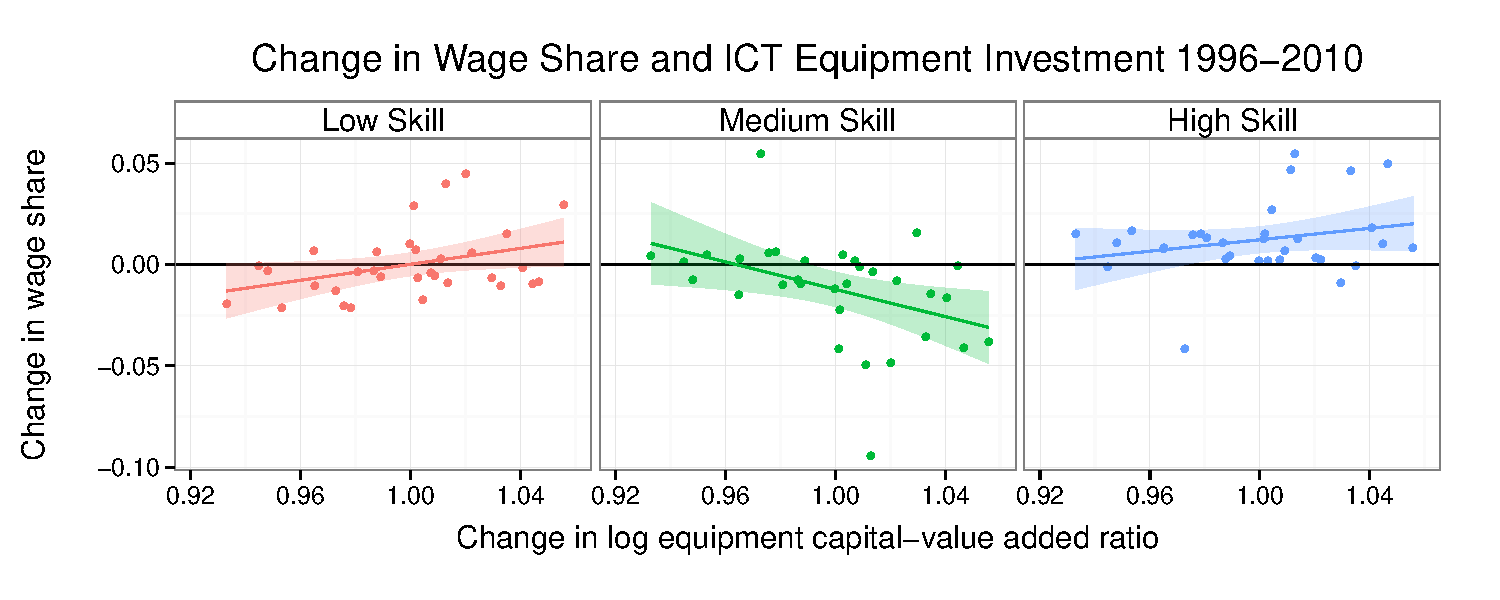
\includegraphics[width=0.8\textwidth]{../figure/wage_share_equipment_skill.pdf}
  \caption{Change in wage share against change in log ICT electrical and electronic equipment capital ratio, by industry, Australia, 1996-2010.
    Trend line shows a LOESS regression with JR kernel and 95\% confidence interval. See note for Table~\ref{tbl:reg} for more details.
  }
  \label{fig:equip}
\end{figure}

\begin{figure}
  \centering
  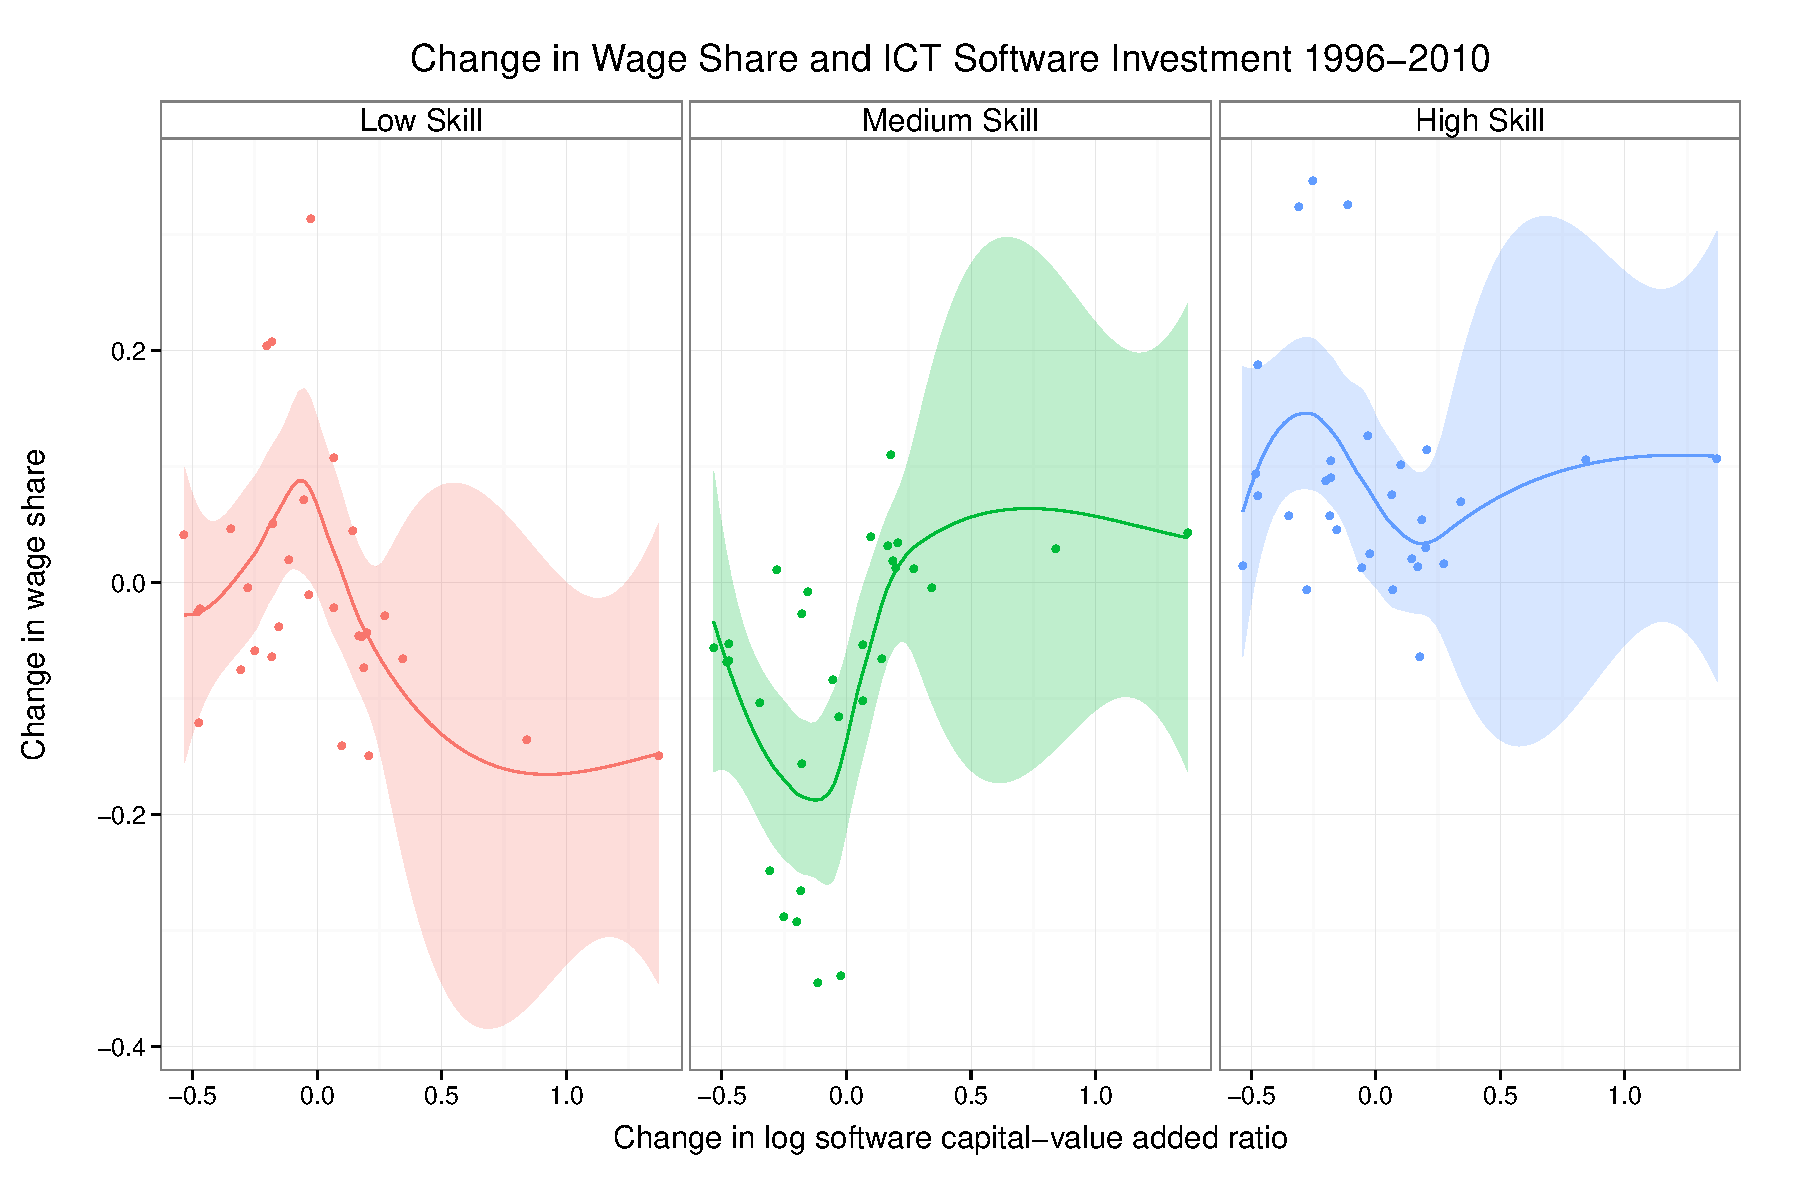
\includegraphics[width=0.8\textwidth]{../figure/wage_share_software_skill.pdf}
  \caption{Change in wage share against change in log ICT software capital ratio, by industry, Australia, 1996-2010.
    See note for Table~\ref{tbl:reg} for more details.
  }
  \label{fig:soft}
\end{figure}

\begin{sidewaystable} \begin{center}
  \caption{Wage Share Change Estimation Results: 1996-2010} 
  \label{tbl:reg} 
\begin{tabular}{@{\extracolsep{5pt}}lcccccc} 
\\[-1.8ex]\hline 
\hline \\[-1.8ex] 
 & \multicolumn{6}{c}{\textit{Dependent variable:}} \\ 
\cline{2-7} 
\\[-1.8ex] & \multicolumn{2}{c}{$\Delta SHARE^H$} & \multicolumn{2}{c}{$\Delta SHARE^M$} & \multicolumn{2}{c}{$\Delta SHARE^L$} \\ 
\\[-1.8ex] & (1) & (2) & (3) & (4) & (5) & (6)\\ 
\hline \\[-1.8ex] 
 $\Delta$log {\em equipment} & 0.037 & 0.081 & $-$0.144 & $-$0.249$^{**}$ & 0.107 & 0.169$^{*}$ \\ 
  & (0.100) & (0.080) & (0.108) & (0.094) & (0.099) & (0.084) \\ 
  & & & & & & \\ 
 $\Delta$log {\em software} & $-$0.018 &  & 0.109$^{*}$ &  & $-$0.091$^{*}$ &  \\ 
  & (0.052) &  & (0.056) &  & (0.052) &  \\ 
  & & & & & & \\ 
 $\Delta$log {\em other capital} & 0.118 &  & $-$0.173 &  & 0.055 &  \\ 
  & (0.176) &  & (0.191) &  & (0.176) &  \\ 
  & & & & & & \\ 
 $\Delta$log {\em value added} & 0.113 & 0.071 & 0.035 & 0.030 & $-$0.148 & $-$0.102 \\ 
  & (0.163) & (0.127) & (0.176) & (0.149) & (0.163) & (0.133) \\ 
  & & & & & & \\ 
 Constant & 0.040 & 0.055 & $-$0.102 & $-$0.095 & 0.062 & 0.040 \\ 
  & (0.073) & (0.060) & (0.079) & (0.070) & (0.073) & (0.063) \\ 
  & & & & & & \\ 
\hline \\[-1.8ex] 
Observations & 30 & 30 & 30 & 30 & 30 & 30 \\ 
R$^{2}$ & 0.068 & 0.044 & 0.343 & 0.210 & 0.251 & 0.151 \\ 
Adjusted R$^{2}$ & $-$0.081 & $-$0.026 & 0.238 & 0.152 & 0.132 & 0.089 \\ 
Residual Std. Error & 0.101 (df = 25) & 0.098 (df = 27) & 0.109 (df = 25) & 0.115 (df = 27) & 0.101 (df = 25) & 0.103 (df = 27) \\ 
F Statistic & 0.455 (df = 4; 25) & 0.627 (df = 2; 27) & 3.268$^{**}$ (df = 4; 25) & 3.593$^{**}$ (df = 2; 27) & 2.100 (df = 4; 25) & 2.409 (df = 2; 27) \\ 
\hline 
\hline \\[-1.8ex] 
\textit{Note:}  & \multicolumn{6}{r}{$^{*}$p$<$0.1; $^{**}$p$<$0.05; $^{***}$p$<$0.01} \\ 
\normalsize 
\end{tabular} 
\end{center}
{\em Wage shares computed for full-time workers, whose primary sources of income are wages and salaries, estimated for 16 industry groups. `High skill' workers include professionals and managers, `middle skill' workers include sales persons, clerical workers and para-professionals, and `low skill' workers include jobs with a high degree of manual activity, including laborers, transport workers and trades persons. To smooth out noise, all variables are estimated in seven-year differences. Survey data are composition adjusted by age bracket, sex and education level to be consistent with 2010 demographics. The variables {\em equipment} and {\em software} respectively refer to the capital stock of electronic and electrical equipment and computer software, at the end of each period. {\em other capital} refers to non-ICT capital, and {\em `value added'} is the value added for that industry group. Source: ABS (Survey of Income and Housing and National Accounts).}
\end{sidewaystable} 

\section{My qualms and questions}\label{qualms}

The model treats ICT capital investment, $C$, as exogenous. However, the middle-skill wage is the price of ICT capital's perfect substitute, and is an endogenous variable. At the margin, the price of both should be equal. But we've assumed the price of labor is uniform. How does one deal with this contradiction? 

ICT investment is a variable that firms select, based on its cost profile: the falling cost of ICT is the entire motivation for the thesis. So if we're going to talk about ICT investment, its price is an important variable.

This also raises the uncomfortable question: exactly how should nominal ICT investment be deflated to give a real capital figure? Cost per computation? Cost per general-purpose computer unit? Equivalized software implementation costs? I suspect this is an unanswerable question, and a good reason to look elsewhere for explanatory variables.

\printbibliography

\end{document}
